\documentclass{article}
\usepackage{graphicx}
\usepackage{float}
\usepackage[top=2 cm, bottom=2 cm, left=2 cm, right=2 cm]{geometry}
\usepackage[sorting=none,
   backend=biber,
   style=alphabetic,
]{biblatex}
\addbibresource{bibliography.bib}
\title{Modeling project: DNA packaging in a virus}
\author{}
\date{October 2023}

\begin{document}

\maketitle

\begin{abstract}
\noindent
In order to infect a host cell, viruses must eject their genome, which is then replicated, followed by the synthesis of the proteins encoded in it. Once the concentration of the proteins is high enough, the construction of the viral capsids, which are rigid protein boxes, is ignited. The next step is the packaging of the viral DNA inside the capsids, which can then be injected into other host cells. The packaging of DNA in viruses is thus an essential step in their life cycle. In this article, we describe a simple physical model explaining this packaging process for the bacteriophage virus $\phi 29$. 
\end{abstract}


\section{Introduction: Orders of magnitudes}
The dynamic of the packing of DNA in a bacteriophage and viruses has been investigated experimentally and theoretically and is now quite elucidated (see \cite{phillips2005} for a complete review). These organisms are forms by a icosahedral capsid that encloses a double stranded beam of DNA. Inside the capsid the DNA is just solvated in an ionic solution. There is no tertiary structure formed of histones and nucleosomes as in eucariot cells. The life cycle of the virus is as follow. It interacts via its spike protein with the membrane of the cell and is able to introduce its genome inside the cell. The DNA of the viruse is then replicated by the cell and expressed to produce the proteins necessary to forme other capsids. The formation of a new viral capsid take typically 10 to 15 minutes for phage $\lambda$ or T4. When a capsid is formed and the genome completely replicated, the portal motor of the capsid, will package the DNA inside the the capsid. This process is typically realised in 5 minutes. After approximately one hour, the cell tends to be full of viruses and dies. This is the lisis that releases the viruses (or phages) in the medium.

The capside has the shape of a sphere or a cylinder with a semi-sphere at each end-cap. WHen the DNA is condensed inside the capsid, it takes the shape of a spool. The strand organise themselves in hexagon with an interstrand space of the order of $25~\AA$ \cite{earnshaw1977}. The capsid radius is smaller than the persistence length of the DNA strand. which means that the DNA is highly constrained inside the capsid. The capsid is impermeable to water. But it is permeable to Polyethilen Glycole (PEG). This property have been used by Evilevitch to apply an osmotic presure against the extraction of the genom of the phage \cite{evilevitch2003}. They report that the ejection of the DNA strand is prevented by a pressure of $20~atm.$

It is believed that the DNA inside the capside organises it self as a spool. But the first experimental measurement of the spatial organisastion of DNA inside the capsid, during the packing process has been observed only in 2008 by Comoli and al. \cite{comoli2008}. They showed that contrarily to what was believed before (for instance in \cite{phillips2005, prohit2005}, DNA tends to organise in the spool structure very late in the packaging process. Until $78\%$ of the genome is packed, the DNA inside the capsides stays in a desordered phase.

\begin{table}[h]
    \centering
    \begin{tabular}{|| r | c | c | l ||}
        \hline \hline
        \textbf{Name of the variable} & \textbf{Symbol} & \textbf{Value} & \textbf{Source} \\
        \hline \hline
        Diameter of the capside  & $d_{cap}$   & $42\times 54~nm$ & Phage $\phi29$ \cite{tao1998}  \\
        Diameter of the dsDNA    & $ d_{dna}$  & $1~nm$           & \cite{phillips2005} \\
        Length of the DNA strand & $ L_{tot}$  & $5.5.10^{3}~nm$  & Phage $\phi29$ \cite{tao1998} \\
        Persistence length       & $ \xi_p $   & $50~m$           & \cite{smith2001} \\
        Gyration radius          & $ R_{G} $     & $300~nm$         & phage $\phi29$ \cite{phillips2005} \\
        Motor force              & $ F_{mot}$  & $10~pN$          & \cite{phillips2005} \\
        Typical pressure         & $ p_{poly}$ & $219~atm.$       & will be explained later \\
        Pressure of non-release  & $ p_{nr} $  & $20~atm.$        & will be explained in the text \\
        \hline \hline
    \end{tabular}
    \caption{Some order of magnitudes about DNA in a viral capsid}
    \label{tab:figures}
\end{table}

\section{Dimensional analysis model}

To understand the relation between the packing percentage and the pressure inside the capsid,, let us start with a small scaling argument. If the DNA is rolled in a spool like structure made of $1$ fold and $N$ hoops in each fold (like a solenoid of $N$ turns). The the length of the DNA in this spool is : $N \sim \frac{L}{2 \pi R}$. Assuming that the interstrand spacing is $r_{IA}$ and assuming that the capsid is a cylinder of height $h$, we typically have $\frac{\sqrt{3}}{2} N r_{IA} \approx h \approx NR$ (assuming that in fact the capsid is almost sperical and $h \sim R$).
An other way to evaluate the scaling law is to suppose that in fact the DNA is almost fully condensed and the cylinder is full of DNA. In this case, if we take a cut of the DNA spool parallel to the axis of the capsid, the surface occupied by DNA is typically: $N \pi r^2_{IA} \sim S$ where $S \sim \pi R^2$. Using once again the fact that $N \sim \frac{L}{2 \pi R}$ we can write $r_{IA} \sim \frac{R^{\frac{3}{2}}}{\sqrt{L}}\sqrt{2}$.
The to deduce a pressure, we use the scaling law that have been pointed out experimentally by Rau et al.: $P \sim e^{-\frac{d_s}{c}}$ (where c is typically just here to addimentionalise $d_s$). We optain the two following scaling laws:
\begin{eqnarray}
    P &\sim& e^{\frac{- 2 \pi R^2}{cL}} \textnormal{ valid for small percentage of packing}\\
    P & \sim & e^{\frac{- \sqrt{2} R^{\frac{3}{2}}}{\sqrt{cL}}} \textnormal{ valid for high percentage of packing} 
\end{eqnarray}
Using the fact that a pressur is proportional to a force time a surface. Here the small surfance of a cut of the DNA, we can try to check our scaling law on the data provided in the subject. We took the points from the graph and ploted the pressure as a function of the inverrse of the percentage of genome packed. We fitted this curve with an exponential function: $x = e^{\gamma x}$. This gives us the result ploted in the figure. To check that the scaling is satisfactory, we can extract back the typical radius of the capsid witch is expressed:
\begin{eqnarray}
    R_{typ} & = &  \sqrt{\frac{\gamma}{2 \pi}} = 6,66 \textnormal{ for the law at low packing density}\\
    R_{typ} & = & 1.414 \gamma^{0.6666} = 32.13 \textnormal{ for the high packaging density}
\end{eqnarray}
We can conclude that at least qualitatively speacking, it seams that the DNA is compact in the denser form we have proposed.

\begin{figure}[H]
    \centering
    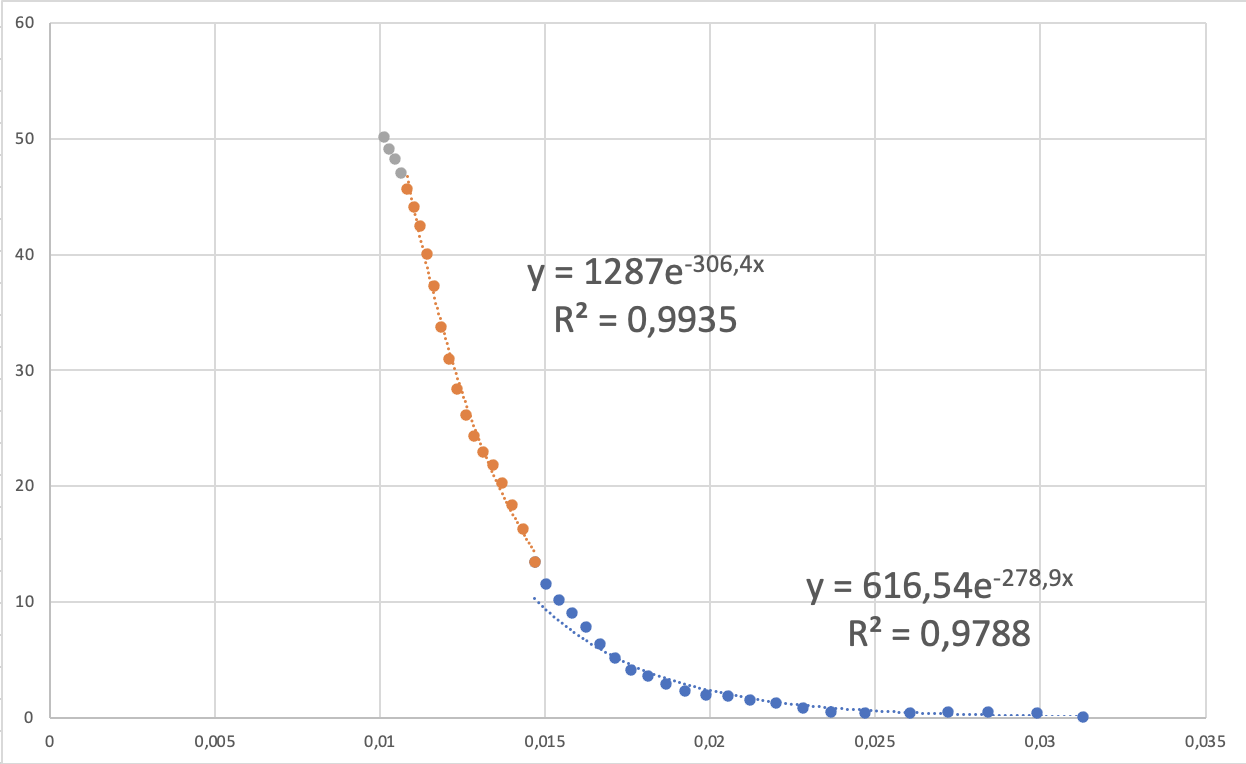
\includegraphics[width=0.8\textwidth]{Fig_Exponents.png}
    \caption{Force of the motor as a function of the percentage of DNA packed. The horizontal axis is the inverse of the percentage of the DNA packed while the vertical axis is the force. We fitted the blue points with the law (1) and the orange points with the law (2). The exponent $\gamma$ of each law can be used to compute the value of the radius of the capsid.}
    \label{fig:force}
\end{figure}

\section{Long polymer model of DNA inside a viral capsid}
An other model that is interesting to unstand the dynamic of a viral capsid is the thermodynamic model of a long polymer under confinement. The idea is simply to use what we know from tutorial 1 about the physics of polymer chains. Which is the following:

\begin{eqnarray}
    G_b & = & \int_{0}^{L} \frac{k_B T \xi_p}{2} \left( \partial_z^2 \mathbf{r}(s) \right)^2 ds
\end{eqnarray}

As the geometry is strongly confined, it is likely that we could not ignore the interaction between the DNA strands. The interaction term of the free energy of this problem can be derives in serveral maner.

\section{Impact of capsid geometry on the packing pressure}

We will study a variety of capsid geometries to assess the impact of this geometry on the packing pressure.

We will first study some simpler geometries analytically, then move to simple numeric analysis.

\begin{figure}[H]
    \centering
    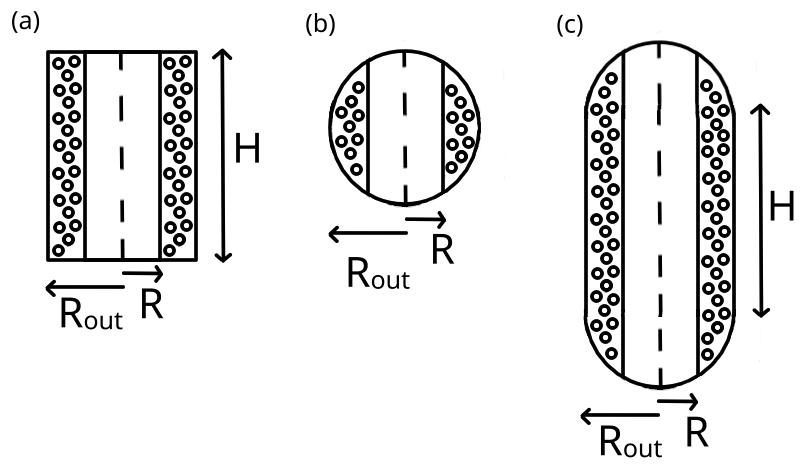
\includegraphics[width=0.7\textwidth]{analitical_geometries.png}
    \caption{Geometries that will be studied analytically: (a) is a simple cylindrical capsid, (b) is a spherical capsid and (c) is a capped cylindrical capsid. We will only model cylindrical and capped cylindrical capsids as spherical capsids can be modeled from a capped-cylindrical capsid with $H=0$}
    \label{fig:enter-label}
\end{figure}

\subsection{Cylindrical capsid}

Blabla....

\subsection{Capped cylindrical capsid}

Blabla....

\subsection{Capsid geometry comparison}

\begin{table}[h]
    \centering
    \begin{tabular}{|| r | c | c | c ||}
        \hline \hline
        \textbf{Name of the variable} & \textbf{cylindrical capsid (a)} & \textbf{spherical capsid (b)} & \textbf{capped cylindrical capsid (c)} \\
        \hline \hline
        Packing section & TODO & TODO & TODO \\
        Packing volume  & TODO & TODO & TODO \\
        Total energy  & TODO & TODO & TODO \\
        Specific energy  & TODO & TODO & TODO \\
        Packing pressure  & TODO & TODO & TODO \\
        \hline \hline
    \end{tabular}
    \caption{Analytical analisis of the various capsid geometries.}
\end{table}

Blabla... 

\subsection{Numerical analysis of the icosahedral capsid geometry}

\begin{figure}[H]
    \centering
    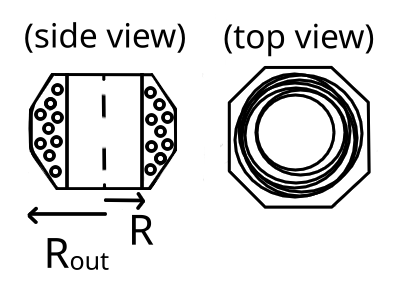
\includegraphics[width=0.4\textwidth]{octogonal_geometry.png}
    \caption{Icosahedral capsid geometry that will be studied numerically.}
    \label{fig:enter-label}
\end{figure}

Although the Icosahedral capsid geometry could be studied analytically, we choose to do a simple numerical analysis as a proof of concept.

We will model (as shown in the top view) that the DNA packs in a circular way parallel to the vertical axis, in a circle of radius equal to the circle that fits inside of the octagonal section of the capsid. We can argue that the DNA will pack this way - at least for "low" packing proportion - to minimise its bending energy, which would be largely increased by the tight bends required to more closely follow the octagonal section of the capsid.


\section{Hestimation of the pressure inside the capsid using the charge of DNA}

Right what I have in my notes.

\section{Entropic Consideractions}
Let us modelise here the DNA as chaine of rods-link representing a polymer. A configuration is fully specified by giving the value of 6 coefficients $(k_i)_{i\in \mathbf{[} 1, 6 \mathbf{]}} $ and $N=\sum_i k_i$
Then the number of configurations is:

\textbf{see page 371 of Phillips}

\textbf{Why is it different from teh expression derived phenomenologicaly in the paper ? Can we bridge teh gap in some manner ?}

\begin{equation}
    W({k_i},N) = \frac{N!}{\prod_{i=1}^6 k_i!}
\end{equation}
And the entropy then reads:

\begin{equation}
     S = - k_B T ln \left( \frac{N!}{\prod_{i=1}^6 k_i!} \right)
\end{equation}

I have never seen this contribution taken into account anywhere. In the fully condensed phase maybe we can neglect it. But whene the DNA is less than 78\% condensed, the disorder might play an important role.

\textbf{It would be great to understand why is it ignored in th papper we have reard ?}

\section{Simple model of viral DNA packing}


\printbibliography[
    heading=bibintoc,
    title={References} ]
\end{document}
